\section{Implementaci\'on de stemming y lematizaci\'on}

Una vez teniendo la lista de palabras \'utiles del texto, se aplicar\'a el m\'etodo de "stemming", el cual consta de reducir a su ra\'iz cada palabra.

Se implementar\'a con ayuda de Snowball, que es un peque\~no lenguaje de programaci\'on para el manejo de strings que nos permite implementar f\'acilmente algoritmos de stemming.

El objetivo de aplicar \'estas dos t\'ecnicas a nuestro corpus de palabras es reducir a\'un m\'as el diccionario de palabras \'utiles eliminando plurales, g\'enero y desinencias verbales, y obteniendo las ra\'ices de todas y cada una de las palabras que obtuvimos de nuestro texto ya eliminadas las stopwords.

El algoritmo de stemming

Las letras en espa\~nol incluyen las siguientes formas acentuadas,

\'a   \'e   \'i   \'o   \'u 

Las siguientes letras son vocales:

a   e   i   o   u   \'a   \'e   \'i   \'o   \'u

R2 es la regi\'on despues de la primer no-vocal que sigue a una vocal en RV, o es la regi\'on nula al final de la palabra si no existe tal no-vocal.

RV es definida a continuaci\'on: 

Si la segunda letra es una consonante, RV es la regi\'on que sigue despues de una vocal, o si las primeras dos letras son vocales, RV es la regi\'on despues de la siguiente consonante, y de otra manera (caso consonante-vocal) RV es la regi\'on despues de la tercera letra. Pero RV es el final de la palabra si aquellas posiciones no son encontradas.

Por ejemplo, 

    m a c h o     o l i v a     t r a b a j o     á u r e o
    
         |...|         |...|         |.......|         |...|
         
Siempre hacer pasos 0 y 1. 

Paso 0: Pronombre

Buscar por el sufijo mas largo entre las siguientes opciones

me   se   sela   selo   selas   selos   la   le   lo   las   les   los   nos

y borrarlo, si viene despues de uno de estos

(a) i\'endo   \'ando   \'ar   \'er   \'ir

(b) ando   iendo   ar   er   ir

(c) yendo despues de una u

en RV. En el caso de (c), yendo debe estar en RV, pero la precedente u puede estar fuera. 

En el caso de (a), el borrado es seguido por remover el acento agudo (por ejemplo, haci\'endola -> haciendo).

Paso 1: Remover sufijos estandar

Buscar el mas largo entre los siguientes sufijos, y realizar la acci\'on indicada. 
anza   anzas   ico   ica   icos   icas   ismo   ismos   able   ables   ible   ibles   ista   istas   oso   osa   osos   osas   amiento   amientos   imiento   imientos

eliminar si en R2

adora   ador   aci\'on   adoras   adores   aciones   ante   antes   ancia   ancias

eliminar si en R2

si es precedido por ic, borrar si en R2 

log\'ia   log\'ias

reemplazar con log si en R2 

uci\'on   uciones

reemplazar con u si en R2 

encia   encias

reemplazar con ente si en R2 

amente

eliminar si en R1

si es precedido por iv, eliminar si en R2 (y si ademas es precedido por at, eliminar si en R2), de otra manera

si es precedido por os, ic o ad, eliminar si en R2 

mente

eliminar si en R2

si es precedido por ante, able or ible, eliminar si en R2 

idad   idades

eliminar si en R2

si es precedido por abil, ic o iv, eliminar si en R2 

iva   ivo   ivas   ivos

eliminar si en R2

si es precedido por at, eliminar si en R2

Hacer paso 2a si ninguna terminación fue removida por el paso 1. 

Paso 2a: Sufijos de verbos iniciando con  y

Buscar por el mas largo entre los siguientes sufijos en RV,  y si es encontrado, eliminar si es precedido por u. 
ya   ye   yan   yen   yeron   yendo   yo   y\'o   yas   yes   yais   yamos

(Nota que la u precedente no necesita estar en  RV.)
Hacer paso2b si paso 2a fue hecho, pero fallo en remover un sufijo. 

Paso 2b: Otros sufijos de verbos

Buscar por el mas largo entre los siguientes sufijos en RV, y realiza la acci\'on indicada. 

en   es   \'eis   emos

eliminar, y si es precedido por gu elimina la u ( gu necesita no estar en RV) 

ar\'ian   ar\'ias   ar\'an   ar\'as   ar\'iais   ar\'ia   ar\'eis   ar\'iamos   aremos   ar\'a   ar\'e   er\'ian   er\'ias   er\'an   er\'as   er\'iais   er\'ia   er\'eis   er\'iamos   eremos   er\'a   er\'e   ir\'ian   ir\'ias   ir\'an   ir\'as   ir\'iais   ir\'ia   ir\'eis   ir\'iamos   iremos   ir\'a   ir\'e   aba   ada   ida   \'ia   ara   iera   ad   ed   id   ase   iese   aste   iste   an   aban   \'ian   aran   ieran   asen   iesen   aron   ieron   ado   ido   ando   iendo   i\'o   ar   er   ir   as   abas   adas   idas   \'ias   aras   ieras   ases   ieses   \'is   \'ais   abais   \'iais   arais   ierais     aseis   ieseis   asteis   isteis   ados   idos   amos   \'abamos   \'iamos   imos   \'aramos   i\'eramos   i\'esemos   \'asemos

eliminar

Siempre hacer paso 3. 

Paso 3: sufijo residual

Buscar por el mas largo entre los siguientes sufijos en RV, y realiza la acción indicada. 

os   a   o   \'a   \'i   \'o

eliminar si en RV 

e   \'e

eliminar si en RV, y si es precedido por gu con la  u en RV eliminar la u

Y finalmente:

Remover acentos

\section{Pruebas}

\subsection{Eliminaci\'on de stopwords}
De acuerdo al diccionario que define las stop words (ver ap\'endice \ref{chap:stop}) al someter por el filtro el texto: ``\textit{Hola hoy es un bonito d\'ia para jugar. Te gustar\'ia venir a mi casa.Nos vamos adivertir a lo grande. Estoy solo mis pap\'as no est\'an.}''. las estop words identificadas de manera manual son: es, un, para, te, a, mi, nos, lo , estoy , no, y est\'an.
Al ser identificadas el algortimo de filtrado las tiene que eliminar de manera autom\'atica.

La figura \ref{elimina_stops} muesta el texto filtrado y con la eliminaci\'on de las palabras identificadas como stopwords.

\begin{figure}
	\begin{center}
		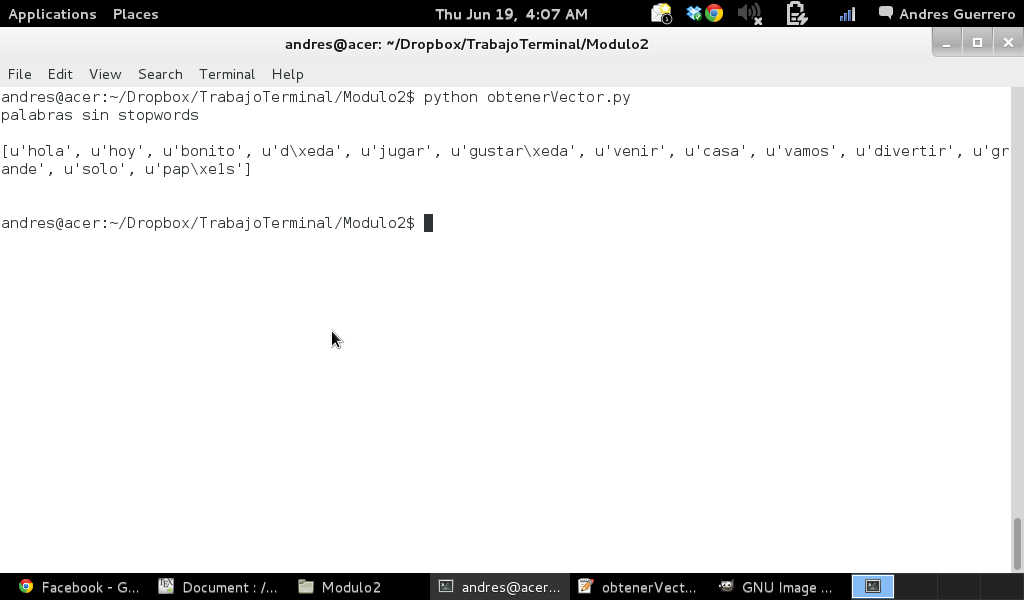
\includegraphics[scale=.4]{images/stopw}
	\end{center}
	 \caption{Ejecuci\'on del filtro de estop words}
	 \label{elimina_stops}
\end{figure}

\subsection{Lematizaci\'on}

Aplicada la prueba anterior al conjunto de palabras resultantes despu\'es del filtrado de stop words aplicando el algoritmo de stemming de manera manual se optienen los siguientes resultados: hol, hoy, bonit, dia, jug, gust,ven,cas vam,divert, grand,sol,papas.

Los resultados obtenidos al implementar el algoritmo de manera autom\'atica se muestran en la figura \ref{stemm}.
\begin{figure}
	\begin{center}
		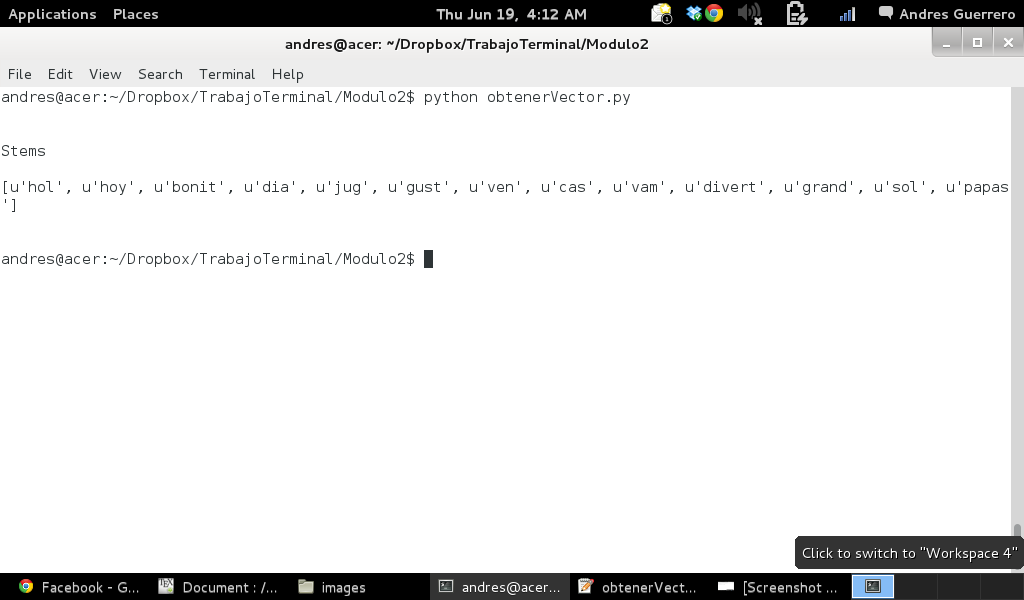
\includegraphics[scale=.4]{images/stemm}
	\end{center}
	 \caption{Ejecuci\'on de implementaci\'on de algoritmo de stemming}
	 \label{stemm}
\end{figure}
